\documentclass[xcolor=svgnames,9pt,english,aspectratio=169,t]{beamer}
%\documentclass[xcolor=svgnames,9pt,english,handout,aspectratio=169,t]{beamer}
\newcommand{\handout}{0}

% =====================================================================
% POLI 450A (2026) --- shared TEMPLATE layer.
%
% Input from each lecture near the top of its file, BEFORE
% ../course_theme.tex (metropolis must be selected before the course
% palette overrides it):
%
%   \documentclass[xcolor=svgnames,9pt,english,aspectratio=169]{beamer}
%   \newcommand{\handout}{0}
%   % =====================================================================
% POLI 450A (2026) --- shared TEMPLATE layer.
%
% Input from each lecture near the top of its file, BEFORE
% ../course_theme.tex (metropolis must be selected before the course
% palette overrides it):
%
%   \documentclass[xcolor=svgnames,9pt,english,aspectratio=169]{beamer}
%   \newcommand{\handout}{0}
%   % =====================================================================
% POLI 450A (2026) --- shared TEMPLATE layer.
%
% Input from each lecture near the top of its file, BEFORE
% ../course_theme.tex (metropolis must be selected before the course
% palette overrides it):
%
%   \documentclass[xcolor=svgnames,9pt,english,aspectratio=169]{beamer}
%   \newcommand{\handout}{0}
%   \input{../course_preamble.tex}
%   \input{../course_theme.tex}
%   \graphicspath{{./}{./figs/}}
%   \title[Short title]{450A Political Methodology I}
%   \subtitle{Lecture N: ...}
%
% Modeled on the 2026 Northwestern workshop template
% (Teaching/PanelData/_latex/2026/202608_Northwestern/workshop_preamble.tex).
%
% SCOPE: theme, beamer layout, packages, the roadmap hooks, and --- unlike
% the Northwestern decks --- the notation macros. The 450A lectures
% grew from one common ancestor, so their macro blocks agree wherever they
% overlap; merging them is safe. Three points where they had drifted are
% resolved here, and each is flagged inline below.
% =====================================================================

\usetheme{metropolis}
\metroset{sectionpage=none, subsectionpage=none, numbering=none}
\setbeamertemplate{navigation symbols}{}

\setbeamersize{text margin left=5mm, text margin right=5mm}
\setbeamertemplate{itemize/enumerate body begin}{\leftmargini=1.5em\relax}
\setbeamertemplate{itemize/enumerate subbody begin}{\leftmarginii=1.5em\relax}
\setbeamertemplate{itemize/enumerate subsubbody begin}{\leftmarginiii=1.5em\relax}

% ----------------------------------------------------------- top alignment
% Every deck passes the t class option, so beamer applies the frame key
% below to every frame (explicit [plain,c] frames — title page, roadmaps —
% stay centered). Beamer's stock t key puts a rigid .2cm pad above the
% content; frames sized to this template's full-height ceilings then run
% Overfull \vbox by up to that pad. Same key as beamerbaseframe.sty, with
% one change: the pad may shrink to zero when the frame is full.
\makeatletter
\define@key{beamerframe}{t}[true]{% top
  \beamer@frametopskip=.2cm plus .5\paperheight minus .2cm\relax%
  \beamer@framebottomskip=0pt plus 1fill\relax%
  \beamer@frametopskipautobreak=\beamer@frametopskip\relax%
  \beamer@framebottomskipautobreak=\beamer@framebottomskip\relax%
}

% ------------------------------------------------- slide-top check (2026-10-11)
% A slide whose content is too tall for the frame is squeezed: the pad above
% shrinks and its content starts higher than on other slides, so a figure
% "wobbles" when the class steps from one slide to the next (Lecture 4-1,
% slides 1-2, 2026-10-11). The marker below records where each slide's
% content starts (a whatsit: it adds no space and moves nothing).
% `python3 ../check_slides.py lec<N>` then lists every slide that starts
% higher than the deck's normal position. That list must be empty.
% Recorded per slide: page, frame number, content-top y (sp), the room left
% below the title bar, and P for a plain frame (title page, roadmaps).
\providecommand\slidetop[5]{}
\AtBeginDocument{\immediate\write\@auxout{\string\providecommand\string\slidetop[5]{}}}
\def\beamer@markframetop{%
  \pdfsavepos
  \edef\beamer@marktmp{\noexpand\write\noexpand\@auxout{\string\slidetop
    {\noexpand\thepage}{\noexpand\insertframenumber}{\noexpand\the\noexpand\pdflastypos}%
    {\number\beamer@frametextheight}{\ifbeamer@plainframe P\else N\fi}}}%
  \beamer@marktmp}
\RequirePackage{etoolbox}
\patchcmd{\endbeamer@frameslide}
  {\vskip\beamer@frametopskip}
  {\vskip\beamer@frametopskip\beamer@markframetop}
  {}{\PackageWarning{course_preamble}{slide-top marker not installed}}
\makeatother

% ---------------------------------------------------------------- packages
\usepackage{xcolor}
\usepackage{colortbl}
\usepackage{amsmath}
\usepackage{amsfonts}
\usepackage{amssymb}
\usepackage{bm}
\usepackage{graphicx}
\usepackage{multirow}
\usepackage{fancyvrb}
\usepackage{listings}
\usepackage{tikz}
\usetikzlibrary{arrows.meta,positioning,decorations.pathreplacing}

% --------------------------------------------------------- figure fitting
% Default bounding box for every \includegraphics that does not override it.
% With keepaspectratio the image is scaled to fit *inside* width x height, so
% a figure can never run past the side margins or off the bottom of a slide.
% Options given at the call site override these on a per-key basis: e.g.
% [width=.6\linewidth] narrows the box but keeps the height ceiling.
% \figmaxheight is set at \begin{document}: beamer only computes the final
% \textheight once the head/foot templates are known. 0.80 is just under what a
% frame with a title and one line of text can hold (measured: 0.834\textheight);
% a frame that needs more room for text can lower it locally.
\newlength{\figmaxheight}
\AtBeginDocument{\setlength{\figmaxheight}{0.80\textheight}}
\setkeys{Gin}{width=\linewidth,height=\figmaxheight,keepaspectratio}

% -------------------------------------------------------- roadmap frames
% Identical in all lectures. A lecture that does not want the
% subsection roadmap clears it after the \input with \AtBeginSubsection[]{}.
% hideothersubsections is load-bearing, not cosmetic: lecture 4 had 13
% subsections before it was split into 4-1, 4-2 and 4-3 (2026-10-09), and a
% full contents list ran off the top and bottom of the slide. Hiding the other sections' subsections caps the list at 10 lines.
\subject{Talks}
% No back-to-back roadmaps (Yiqing, 2026-10-11): when a subsection starts right
% after its section's roadmap, with no content slide in between, its own
% roadmap would repeat the one just shown (5-1's handout showed "Two Cases"
% twice), so it is skipped. The section roadmap records the frame count; the
% subsection roadmap appears only if a content slide has come since.
\makeatletter
\def\course@secframe{-1}
\AtBeginSection[]
{
  \begin{frame}[plain,c]
    \frametitle{}
    \tableofcontents[currentsection,hideothersubsections]
    \addtocounter{framenumber}{-1}
  \end{frame}
  \xdef\course@secframe{\the\c@framenumber}
}
\AtBeginSubsection[]
{
  \ifnum\c@framenumber=\course@secframe\relax\else
  \begin{frame}[plain,c]
    \frametitle{}
    \tableofcontents[currentsection,currentsubsection,hideothersubsections]
    \addtocounter{framenumber}{-1}
  \end{frame}
  \fi
}
\makeatother

% ------------------------------------------------------ theorem environments
\newtheorem{assumption}{Assumption}
\newtheorem{iass}{Identification Assumption}
\newtheorem{ires}{Identification Result}
\newtheorem{estm}{Estimand}
\newtheorem{esti}{Estimator}
\newtheorem{question}{Question}
\newtheorem{answer}{Answer}
\newtheorem{proposition}{Proposition}

% =====================================================================
% Notation
% =====================================================================
\definecolor{dgreen}{rgb}{0,.6,0.8}

\renewcommand\r{\right}
\renewcommand\l{\left}
\newcommand{\bs}{\boldsymbol}
\newcommand{\mb}{\mathbf}
\newcommand{\real}{\mathbb{R}}
\newcommand{\cN}{\mathcal{N}}
\newcommand{\E}{\mathbb{E}}
\newcommand{\V}{\mathbb{V}}

% MERGE NOTE 1. Lecture 2-4 set \epsilon to \varepsilon; the other twelve
% left it at the upright default. Adopting \varepsilon course-wide so the
% error term looks the same in every lecture.
\renewcommand{\epsilon}{\varepsilon}

% MERGE NOTE 2. Lecture 2-4 wrote its vectors as \bm (bold italic); the other
% twelve use \mathbf (bold upright). \mathbf wins --- it is the convention in
% eleven of the thirteen decks and in the course's matrix lectures. Only
% \iid, \E, \cN and \Var from that block are actually used in 2-4's body.
\renewcommand{\u}{\ensuremath{\mb{u}}}
\renewcommand{\v}{\ensuremath{\mb{v}}}
\newcommand{\U}{\ensuremath{\mb{U}}}
\newcommand{\M}{\ensuremath{\mb{M}}}
\newcommand{\X}{\ensuremath{\mb{X}}}
\newcommand{\x}{\ensuremath{\mb{x}}}
\newcommand{\y}{\ensuremath{\mb{y}}}
\newcommand{\Z}{\ensuremath{\mb{Z}}}
\newcommand{\C}{\ensuremath{\mb{C}}}
\newcommand{\D}{\ensuremath{\mb{D}}}
\newcommand{\I}{\ensuremath{\mb{I}}}
\newcommand{\W}{\ensuremath{\mb{W}}}
\renewcommand{\a}{\ensuremath{\mb{a}}}
\renewcommand{\P}{\ensuremath{\mb{P}}}
\newcommand{\one}{\ensuremath{\mb{1}}}
\newcommand{\zero}{\ensuremath{\mb{0}}}

\renewcommand{\b}{\ensuremath{\bs{\beta}}}
\newcommand{\be}{\ensuremath{\bs{\beta}}}
\newcommand{\e}{\ensuremath{\bs{\epsilon}}}
\newcommand{\eps}{\ensuremath{\bs{\epsilon}}}
\newcommand{\eeta}{\ensuremath{\bs{\eta}}}
\newcommand{\bhat}{\ensuremath{\hat{\bs{\beta}}}}
\newcommand{\ehat}{\ensuremath{\hat{\e}}}
\newcommand{\Sig}{\ensuremath{\bs{\Sigma}}}
\newcommand{\SigInv}{\ensuremath{\bs{\Sigma^{-1}}}}

\newcommand{\XX}{\ensuremath{\X'\X}}
\newcommand{\XXinv}{\ensuremath{\left(\XX\right)^{-1}}}
\newcommand{\hatmat}{\ensuremath{\X \XXinv \X'}}
\newcommand{\hatsig}{\ensuremath{\hat{\sigma}^2}}
\newcommand{\sig}{\ensuremath{\sigma^2}}

\newcommand{\cA}{\mathcal{A}}
\newcommand{\cJ}{\mathcal{J}}
\newcommand{\cL}{\mathcal{L}}
\newcommand{\cLL}{\mathcal{LL}}
\newcommand{\cll}{\ell}
\newcommand{\cQ}{\mathcal{Q}}
\newcommand{\cP}{\mathcal{P}}

% MERGE NOTE 3. \var / \Var and \cov / \Cov were spelled with \text in some
% lectures and \mbox in others. Same output; \text kept.
\newcommand{\var}{\text{Var}}
\newcommand{\Var}{\text{Var}}
\newcommand{\cov}{\text{Cov}}
\newcommand{\Cov}{\text{Cov}}
\newcommand{\cor}{\text{Cor}}
\newcommand{\tr}{\text{tr}}
\newcommand{\avepop}{\frac{1}{n}\sum_{i=1}^n}

\DeclareMathOperator*\plim{plim}
\DeclareMathOperator\rank{rank}
\DeclareMathOperator*\argmax{argmax}
\DeclareMathOperator*\argmin{argmin}
\DeclareMathOperator{\sgn}{sgn}
\newcommand{\diag}{\mathop{\mathrm{diag}}}

\newcommand\ud{\mathrm{d}}
\newcommand\dist{\buildrel\rm d\over\sim}
\newcommand\ind{\stackrel{\rm indep.}{\sim}}
\newcommand\iid{\stackrel{\rm i.i.d.}{\sim}}
\newcommand\logit{{\rm logit}}

\newcommand\indep{\protect\mathpalette{\protect\independenT}{\perp}}
\def\independenT#1#2{\mathrel{\rlap{$#1#2$}\mkern2mu{#1#2}}}

% ------------------------------------------------------------- text helpers
\newcommand{\bi}{\begin{itemize}}
\newcommand{\ei}{\end{itemize}}
\newcommand{\noi}{\noindent}
\newcommand{\red}{\textcolor{Cardinal}}
\newcommand{\blue}{\textcolor{CourseBlue}}
\newcommand{\gray}{\textcolor{gray}}
\newcommand\spacingset[1]{\renewcommand{\baselinestretch}{#1}\small\normalsize}

\hyphenation{tyamamot}


% ------------------------------------------------ figure-position check (2026-10-11)
% Records where every \includegraphics lands and its size (a whatsit; it moves
% nothing). check_slides.py flags two consecutive slides that show a figure of
% the same size in different places: the class sees it jump (Lecture 3, slides
% 18 to 19: one frame had \vspace{.3cm} above the figure, the next did not),
% and two consecutive slides that show the same file at different sizes or
% places (Lecture 6-3, slides 10 to 11, the ballot image). The file name is the
% seventh field.
\makeatletter
\providecommand\figpos[7]{}
\AtBeginDocument{\immediate\write\@auxout{\string\providecommand\string\figpos[7]{}}}
\newbox\course@figbox
\let\course@origGinclude\Ginclude@graphics
\def\Ginclude@graphics#1{%
  \setbox\course@figbox\hbox{\course@origGinclude{#1}}%
  \pdfsavepos
  \edef\course@figtmp{\noexpand\write\noexpand\@auxout{\string\figpos
    {\noexpand\thepage}{\noexpand\insertframenumber}%
    {\noexpand\the\noexpand\pdflastxpos}{\noexpand\the\noexpand\pdflastypos}%
    {\number\wd\course@figbox}{\number\ht\course@figbox}{\detokenize{#1}}}}%
  \course@figtmp
  \box\course@figbox}
\makeatother

%   % =====================================================================
% POLI 450A (2026) --- shared visual system.
% Input from each lecture AFTER ../course_preamble.tex.
%
% Same shape as the 2026 Northwestern workshop theme
% (Teaching/PanelData/_latex/2026/202608_Northwestern/workshop_theme.tex),
% with the workshop's purple swapped for the course's cardinal. Kept
% deliberately light so the lecture sources stay easy to edit.
%
% To retune the course to Stanford's official cardinal, change the one
% Cardinal line below to HTML 8C1515.
% =====================================================================
\definecolor{Cardinal}{HTML}{A8003B}     % primary: titles, structure, alerts
\definecolor{CourseInk}{HTML}{252A34}    % body text
\definecolor{CourseBlue}{HTML}{2F6B9A}   % secondary accent
\definecolor{CourseMist}{HTML}{F8F1F4}   % block backgrounds

\setbeamercolor{normal text}{fg=CourseInk,bg=white}
\setbeamercolor{structure}{fg=Cardinal}
\setbeamercolor{alerted text}{fg=Cardinal}
\setbeamercolor{frametitle}{fg=white,bg=Cardinal}
\setbeamercolor{title}{fg=Cardinal}
\setbeamercolor{subtitle}{fg=CourseInk}
\setbeamercolor{block title}{fg=white,bg=Cardinal}
\setbeamercolor{block body}{fg=CourseInk,bg=CourseMist}
\setbeamercolor{section in toc}{fg=Cardinal}
\setbeamercolor{subsection in toc}{fg=CourseInk}
\setbeamercolor{itemize item}{fg=Cardinal}
\setbeamercolor{itemize subitem}{fg=Cardinal}
\setbeamercolor{enumerate item}{fg=Cardinal}

\setbeamerfont{title}{series=\bfseries,size=\Large}
\setbeamerfont{frametitle}{series=\bfseries,size=\large}
\setbeamerfont{block title}{series=\bfseries}
\setbeamertemplate{navigation symbols}{}
\setbeamertemplate{items}[circle]
\setbeamertemplate{blocks}[rounded][shadow=false]
\setbeamertemplate{frametitle continuation}{}
\setbeamertemplate{footline}{%
  \leavevmode\hbox{%
  \begin{beamercolorbox}[wd=.88\paperwidth,ht=2.6ex,dp=1.2ex,leftskip=1.2em]{author in head/foot}%
  \usebeamerfont{author in head/foot}\insertshorttitle
  \end{beamercolorbox}%
  \begin{beamercolorbox}[wd=.12\paperwidth,ht=2.6ex,dp=1.2ex,center]{date in head/foot}%
  \insertframenumber
  \end{beamercolorbox}}}

\newcommand{\slidesource}[1]{\vfill{\scriptsize\color{gray}Source: #1}}
\newcommand{\keyquestion}[1]{\begin{block}{Question}#1\end{block}}

%   \graphicspath{{./}{./figs/}}
%   \title[Short title]{450A Political Methodology I}
%   \subtitle{Lecture N: ...}
%
% Modeled on the 2026 Northwestern workshop template
% (Teaching/PanelData/_latex/2026/202608_Northwestern/workshop_preamble.tex).
%
% SCOPE: theme, beamer layout, packages, the roadmap hooks, and --- unlike
% the Northwestern decks --- the notation macros. The 450A lectures
% grew from one common ancestor, so their macro blocks agree wherever they
% overlap; merging them is safe. Three points where they had drifted are
% resolved here, and each is flagged inline below.
% =====================================================================

\usetheme{metropolis}
\metroset{sectionpage=none, subsectionpage=none, numbering=none}
\setbeamertemplate{navigation symbols}{}

\setbeamersize{text margin left=5mm, text margin right=5mm}
\setbeamertemplate{itemize/enumerate body begin}{\leftmargini=1.5em\relax}
\setbeamertemplate{itemize/enumerate subbody begin}{\leftmarginii=1.5em\relax}
\setbeamertemplate{itemize/enumerate subsubbody begin}{\leftmarginiii=1.5em\relax}

% ----------------------------------------------------------- top alignment
% Every deck passes the t class option, so beamer applies the frame key
% below to every frame (explicit [plain,c] frames — title page, roadmaps —
% stay centered). Beamer's stock t key puts a rigid .2cm pad above the
% content; frames sized to this template's full-height ceilings then run
% Overfull \vbox by up to that pad. Same key as beamerbaseframe.sty, with
% one change: the pad may shrink to zero when the frame is full.
\makeatletter
\define@key{beamerframe}{t}[true]{% top
  \beamer@frametopskip=.2cm plus .5\paperheight minus .2cm\relax%
  \beamer@framebottomskip=0pt plus 1fill\relax%
  \beamer@frametopskipautobreak=\beamer@frametopskip\relax%
  \beamer@framebottomskipautobreak=\beamer@framebottomskip\relax%
}

% ------------------------------------------------- slide-top check (2026-10-11)
% A slide whose content is too tall for the frame is squeezed: the pad above
% shrinks and its content starts higher than on other slides, so a figure
% "wobbles" when the class steps from one slide to the next (Lecture 4-1,
% slides 1-2, 2026-10-11). The marker below records where each slide's
% content starts (a whatsit: it adds no space and moves nothing).
% `python3 ../check_slides.py lec<N>` then lists every slide that starts
% higher than the deck's normal position. That list must be empty.
% Recorded per slide: page, frame number, content-top y (sp), the room left
% below the title bar, and P for a plain frame (title page, roadmaps).
\providecommand\slidetop[5]{}
\AtBeginDocument{\immediate\write\@auxout{\string\providecommand\string\slidetop[5]{}}}
\def\beamer@markframetop{%
  \pdfsavepos
  \edef\beamer@marktmp{\noexpand\write\noexpand\@auxout{\string\slidetop
    {\noexpand\thepage}{\noexpand\insertframenumber}{\noexpand\the\noexpand\pdflastypos}%
    {\number\beamer@frametextheight}{\ifbeamer@plainframe P\else N\fi}}}%
  \beamer@marktmp}
\RequirePackage{etoolbox}
\patchcmd{\endbeamer@frameslide}
  {\vskip\beamer@frametopskip}
  {\vskip\beamer@frametopskip\beamer@markframetop}
  {}{\PackageWarning{course_preamble}{slide-top marker not installed}}
\makeatother

% ---------------------------------------------------------------- packages
\usepackage{xcolor}
\usepackage{colortbl}
\usepackage{amsmath}
\usepackage{amsfonts}
\usepackage{amssymb}
\usepackage{bm}
\usepackage{graphicx}
\usepackage{multirow}
\usepackage{fancyvrb}
\usepackage{listings}
\usepackage{tikz}
\usetikzlibrary{arrows.meta,positioning,decorations.pathreplacing}

% --------------------------------------------------------- figure fitting
% Default bounding box for every \includegraphics that does not override it.
% With keepaspectratio the image is scaled to fit *inside* width x height, so
% a figure can never run past the side margins or off the bottom of a slide.
% Options given at the call site override these on a per-key basis: e.g.
% [width=.6\linewidth] narrows the box but keeps the height ceiling.
% \figmaxheight is set at \begin{document}: beamer only computes the final
% \textheight once the head/foot templates are known. 0.80 is just under what a
% frame with a title and one line of text can hold (measured: 0.834\textheight);
% a frame that needs more room for text can lower it locally.
\newlength{\figmaxheight}
\AtBeginDocument{\setlength{\figmaxheight}{0.80\textheight}}
\setkeys{Gin}{width=\linewidth,height=\figmaxheight,keepaspectratio}

% -------------------------------------------------------- roadmap frames
% Identical in all lectures. A lecture that does not want the
% subsection roadmap clears it after the \input with \AtBeginSubsection[]{}.
% hideothersubsections is load-bearing, not cosmetic: lecture 4 had 13
% subsections before it was split into 4-1, 4-2 and 4-3 (2026-10-09), and a
% full contents list ran off the top and bottom of the slide. Hiding the other sections' subsections caps the list at 10 lines.
\subject{Talks}
% No back-to-back roadmaps (Yiqing, 2026-10-11): when a subsection starts right
% after its section's roadmap, with no content slide in between, its own
% roadmap would repeat the one just shown (5-1's handout showed "Two Cases"
% twice), so it is skipped. The section roadmap records the frame count; the
% subsection roadmap appears only if a content slide has come since.
\makeatletter
\def\course@secframe{-1}
\AtBeginSection[]
{
  \begin{frame}[plain,c]
    \frametitle{}
    \tableofcontents[currentsection,hideothersubsections]
    \addtocounter{framenumber}{-1}
  \end{frame}
  \xdef\course@secframe{\the\c@framenumber}
}
\AtBeginSubsection[]
{
  \ifnum\c@framenumber=\course@secframe\relax\else
  \begin{frame}[plain,c]
    \frametitle{}
    \tableofcontents[currentsection,currentsubsection,hideothersubsections]
    \addtocounter{framenumber}{-1}
  \end{frame}
  \fi
}
\makeatother

% ------------------------------------------------------ theorem environments
\newtheorem{assumption}{Assumption}
\newtheorem{iass}{Identification Assumption}
\newtheorem{ires}{Identification Result}
\newtheorem{estm}{Estimand}
\newtheorem{esti}{Estimator}
\newtheorem{question}{Question}
\newtheorem{answer}{Answer}
\newtheorem{proposition}{Proposition}

% =====================================================================
% Notation
% =====================================================================
\definecolor{dgreen}{rgb}{0,.6,0.8}

\renewcommand\r{\right}
\renewcommand\l{\left}
\newcommand{\bs}{\boldsymbol}
\newcommand{\mb}{\mathbf}
\newcommand{\real}{\mathbb{R}}
\newcommand{\cN}{\mathcal{N}}
\newcommand{\E}{\mathbb{E}}
\newcommand{\V}{\mathbb{V}}

% MERGE NOTE 1. Lecture 2-4 set \epsilon to \varepsilon; the other twelve
% left it at the upright default. Adopting \varepsilon course-wide so the
% error term looks the same in every lecture.
\renewcommand{\epsilon}{\varepsilon}

% MERGE NOTE 2. Lecture 2-4 wrote its vectors as \bm (bold italic); the other
% twelve use \mathbf (bold upright). \mathbf wins --- it is the convention in
% eleven of the thirteen decks and in the course's matrix lectures. Only
% \iid, \E, \cN and \Var from that block are actually used in 2-4's body.
\renewcommand{\u}{\ensuremath{\mb{u}}}
\renewcommand{\v}{\ensuremath{\mb{v}}}
\newcommand{\U}{\ensuremath{\mb{U}}}
\newcommand{\M}{\ensuremath{\mb{M}}}
\newcommand{\X}{\ensuremath{\mb{X}}}
\newcommand{\x}{\ensuremath{\mb{x}}}
\newcommand{\y}{\ensuremath{\mb{y}}}
\newcommand{\Z}{\ensuremath{\mb{Z}}}
\newcommand{\C}{\ensuremath{\mb{C}}}
\newcommand{\D}{\ensuremath{\mb{D}}}
\newcommand{\I}{\ensuremath{\mb{I}}}
\newcommand{\W}{\ensuremath{\mb{W}}}
\renewcommand{\a}{\ensuremath{\mb{a}}}
\renewcommand{\P}{\ensuremath{\mb{P}}}
\newcommand{\one}{\ensuremath{\mb{1}}}
\newcommand{\zero}{\ensuremath{\mb{0}}}

\renewcommand{\b}{\ensuremath{\bs{\beta}}}
\newcommand{\be}{\ensuremath{\bs{\beta}}}
\newcommand{\e}{\ensuremath{\bs{\epsilon}}}
\newcommand{\eps}{\ensuremath{\bs{\epsilon}}}
\newcommand{\eeta}{\ensuremath{\bs{\eta}}}
\newcommand{\bhat}{\ensuremath{\hat{\bs{\beta}}}}
\newcommand{\ehat}{\ensuremath{\hat{\e}}}
\newcommand{\Sig}{\ensuremath{\bs{\Sigma}}}
\newcommand{\SigInv}{\ensuremath{\bs{\Sigma^{-1}}}}

\newcommand{\XX}{\ensuremath{\X'\X}}
\newcommand{\XXinv}{\ensuremath{\left(\XX\right)^{-1}}}
\newcommand{\hatmat}{\ensuremath{\X \XXinv \X'}}
\newcommand{\hatsig}{\ensuremath{\hat{\sigma}^2}}
\newcommand{\sig}{\ensuremath{\sigma^2}}

\newcommand{\cA}{\mathcal{A}}
\newcommand{\cJ}{\mathcal{J}}
\newcommand{\cL}{\mathcal{L}}
\newcommand{\cLL}{\mathcal{LL}}
\newcommand{\cll}{\ell}
\newcommand{\cQ}{\mathcal{Q}}
\newcommand{\cP}{\mathcal{P}}

% MERGE NOTE 3. \var / \Var and \cov / \Cov were spelled with \text in some
% lectures and \mbox in others. Same output; \text kept.
\newcommand{\var}{\text{Var}}
\newcommand{\Var}{\text{Var}}
\newcommand{\cov}{\text{Cov}}
\newcommand{\Cov}{\text{Cov}}
\newcommand{\cor}{\text{Cor}}
\newcommand{\tr}{\text{tr}}
\newcommand{\avepop}{\frac{1}{n}\sum_{i=1}^n}

\DeclareMathOperator*\plim{plim}
\DeclareMathOperator\rank{rank}
\DeclareMathOperator*\argmax{argmax}
\DeclareMathOperator*\argmin{argmin}
\DeclareMathOperator{\sgn}{sgn}
\newcommand{\diag}{\mathop{\mathrm{diag}}}

\newcommand\ud{\mathrm{d}}
\newcommand\dist{\buildrel\rm d\over\sim}
\newcommand\ind{\stackrel{\rm indep.}{\sim}}
\newcommand\iid{\stackrel{\rm i.i.d.}{\sim}}
\newcommand\logit{{\rm logit}}

\newcommand\indep{\protect\mathpalette{\protect\independenT}{\perp}}
\def\independenT#1#2{\mathrel{\rlap{$#1#2$}\mkern2mu{#1#2}}}

% ------------------------------------------------------------- text helpers
\newcommand{\bi}{\begin{itemize}}
\newcommand{\ei}{\end{itemize}}
\newcommand{\noi}{\noindent}
\newcommand{\red}{\textcolor{Cardinal}}
\newcommand{\blue}{\textcolor{CourseBlue}}
\newcommand{\gray}{\textcolor{gray}}
\newcommand\spacingset[1]{\renewcommand{\baselinestretch}{#1}\small\normalsize}

\hyphenation{tyamamot}


% ------------------------------------------------ figure-position check (2026-10-11)
% Records where every \includegraphics lands and its size (a whatsit; it moves
% nothing). check_slides.py flags two consecutive slides that show a figure of
% the same size in different places: the class sees it jump (Lecture 3, slides
% 18 to 19: one frame had \vspace{.3cm} above the figure, the next did not),
% and two consecutive slides that show the same file at different sizes or
% places (Lecture 6-3, slides 10 to 11, the ballot image). The file name is the
% seventh field.
\makeatletter
\providecommand\figpos[7]{}
\AtBeginDocument{\immediate\write\@auxout{\string\providecommand\string\figpos[7]{}}}
\newbox\course@figbox
\let\course@origGinclude\Ginclude@graphics
\def\Ginclude@graphics#1{%
  \setbox\course@figbox\hbox{\course@origGinclude{#1}}%
  \pdfsavepos
  \edef\course@figtmp{\noexpand\write\noexpand\@auxout{\string\figpos
    {\noexpand\thepage}{\noexpand\insertframenumber}%
    {\noexpand\the\noexpand\pdflastxpos}{\noexpand\the\noexpand\pdflastypos}%
    {\number\wd\course@figbox}{\number\ht\course@figbox}{\detokenize{#1}}}}%
  \course@figtmp
  \box\course@figbox}
\makeatother

%   % =====================================================================
% POLI 450A (2026) --- shared visual system.
% Input from each lecture AFTER ../course_preamble.tex.
%
% Same shape as the 2026 Northwestern workshop theme
% (Teaching/PanelData/_latex/2026/202608_Northwestern/workshop_theme.tex),
% with the workshop's purple swapped for the course's cardinal. Kept
% deliberately light so the lecture sources stay easy to edit.
%
% To retune the course to Stanford's official cardinal, change the one
% Cardinal line below to HTML 8C1515.
% =====================================================================
\definecolor{Cardinal}{HTML}{A8003B}     % primary: titles, structure, alerts
\definecolor{CourseInk}{HTML}{252A34}    % body text
\definecolor{CourseBlue}{HTML}{2F6B9A}   % secondary accent
\definecolor{CourseMist}{HTML}{F8F1F4}   % block backgrounds

\setbeamercolor{normal text}{fg=CourseInk,bg=white}
\setbeamercolor{structure}{fg=Cardinal}
\setbeamercolor{alerted text}{fg=Cardinal}
\setbeamercolor{frametitle}{fg=white,bg=Cardinal}
\setbeamercolor{title}{fg=Cardinal}
\setbeamercolor{subtitle}{fg=CourseInk}
\setbeamercolor{block title}{fg=white,bg=Cardinal}
\setbeamercolor{block body}{fg=CourseInk,bg=CourseMist}
\setbeamercolor{section in toc}{fg=Cardinal}
\setbeamercolor{subsection in toc}{fg=CourseInk}
\setbeamercolor{itemize item}{fg=Cardinal}
\setbeamercolor{itemize subitem}{fg=Cardinal}
\setbeamercolor{enumerate item}{fg=Cardinal}

\setbeamerfont{title}{series=\bfseries,size=\Large}
\setbeamerfont{frametitle}{series=\bfseries,size=\large}
\setbeamerfont{block title}{series=\bfseries}
\setbeamertemplate{navigation symbols}{}
\setbeamertemplate{items}[circle]
\setbeamertemplate{blocks}[rounded][shadow=false]
\setbeamertemplate{frametitle continuation}{}
\setbeamertemplate{footline}{%
  \leavevmode\hbox{%
  \begin{beamercolorbox}[wd=.88\paperwidth,ht=2.6ex,dp=1.2ex,leftskip=1.2em]{author in head/foot}%
  \usebeamerfont{author in head/foot}\insertshorttitle
  \end{beamercolorbox}%
  \begin{beamercolorbox}[wd=.12\paperwidth,ht=2.6ex,dp=1.2ex,center]{date in head/foot}%
  \insertframenumber
  \end{beamercolorbox}}}

\newcommand{\slidesource}[1]{\vfill{\scriptsize\color{gray}Source: #1}}
\newcommand{\keyquestion}[1]{\begin{block}{Question}#1\end{block}}

%   \graphicspath{{./}{./figs/}}
%   \title[Short title]{450A Political Methodology I}
%   \subtitle{Lecture N: ...}
%
% Modeled on the 2026 Northwestern workshop template
% (Teaching/PanelData/_latex/2026/202608_Northwestern/workshop_preamble.tex).
%
% SCOPE: theme, beamer layout, packages, the roadmap hooks, and --- unlike
% the Northwestern decks --- the notation macros. The 450A lectures
% grew from one common ancestor, so their macro blocks agree wherever they
% overlap; merging them is safe. Three points where they had drifted are
% resolved here, and each is flagged inline below.
% =====================================================================

\usetheme{metropolis}
\metroset{sectionpage=none, subsectionpage=none, numbering=none}
\setbeamertemplate{navigation symbols}{}

\setbeamersize{text margin left=5mm, text margin right=5mm}
\setbeamertemplate{itemize/enumerate body begin}{\leftmargini=1.5em\relax}
\setbeamertemplate{itemize/enumerate subbody begin}{\leftmarginii=1.5em\relax}
\setbeamertemplate{itemize/enumerate subsubbody begin}{\leftmarginiii=1.5em\relax}

% ----------------------------------------------------------- top alignment
% Every deck passes the t class option, so beamer applies the frame key
% below to every frame (explicit [plain,c] frames — title page, roadmaps —
% stay centered). Beamer's stock t key puts a rigid .2cm pad above the
% content; frames sized to this template's full-height ceilings then run
% Overfull \vbox by up to that pad. Same key as beamerbaseframe.sty, with
% one change: the pad may shrink to zero when the frame is full.
\makeatletter
\define@key{beamerframe}{t}[true]{% top
  \beamer@frametopskip=.2cm plus .5\paperheight minus .2cm\relax%
  \beamer@framebottomskip=0pt plus 1fill\relax%
  \beamer@frametopskipautobreak=\beamer@frametopskip\relax%
  \beamer@framebottomskipautobreak=\beamer@framebottomskip\relax%
}

% ------------------------------------------------- slide-top check (2026-10-11)
% A slide whose content is too tall for the frame is squeezed: the pad above
% shrinks and its content starts higher than on other slides, so a figure
% "wobbles" when the class steps from one slide to the next (Lecture 4-1,
% slides 1-2, 2026-10-11). The marker below records where each slide's
% content starts (a whatsit: it adds no space and moves nothing).
% `python3 ../check_slides.py lec<N>` then lists every slide that starts
% higher than the deck's normal position. That list must be empty.
% Recorded per slide: page, frame number, content-top y (sp), the room left
% below the title bar, and P for a plain frame (title page, roadmaps).
\providecommand\slidetop[5]{}
\AtBeginDocument{\immediate\write\@auxout{\string\providecommand\string\slidetop[5]{}}}
\def\beamer@markframetop{%
  \pdfsavepos
  \edef\beamer@marktmp{\noexpand\write\noexpand\@auxout{\string\slidetop
    {\noexpand\thepage}{\noexpand\insertframenumber}{\noexpand\the\noexpand\pdflastypos}%
    {\number\beamer@frametextheight}{\ifbeamer@plainframe P\else N\fi}}}%
  \beamer@marktmp}
\RequirePackage{etoolbox}
\patchcmd{\endbeamer@frameslide}
  {\vskip\beamer@frametopskip}
  {\vskip\beamer@frametopskip\beamer@markframetop}
  {}{\PackageWarning{course_preamble}{slide-top marker not installed}}
\makeatother

% ---------------------------------------------------------------- packages
\usepackage{xcolor}
\usepackage{colortbl}
\usepackage{amsmath}
\usepackage{amsfonts}
\usepackage{amssymb}
\usepackage{bm}
\usepackage{graphicx}
\usepackage{multirow}
\usepackage{fancyvrb}
\usepackage{listings}
\usepackage{tikz}
\usetikzlibrary{arrows.meta,positioning,decorations.pathreplacing}

% --------------------------------------------------------- figure fitting
% Default bounding box for every \includegraphics that does not override it.
% With keepaspectratio the image is scaled to fit *inside* width x height, so
% a figure can never run past the side margins or off the bottom of a slide.
% Options given at the call site override these on a per-key basis: e.g.
% [width=.6\linewidth] narrows the box but keeps the height ceiling.
% \figmaxheight is set at \begin{document}: beamer only computes the final
% \textheight once the head/foot templates are known. 0.80 is just under what a
% frame with a title and one line of text can hold (measured: 0.834\textheight);
% a frame that needs more room for text can lower it locally.
\newlength{\figmaxheight}
\AtBeginDocument{\setlength{\figmaxheight}{0.80\textheight}}
\setkeys{Gin}{width=\linewidth,height=\figmaxheight,keepaspectratio}

% -------------------------------------------------------- roadmap frames
% Identical in all lectures. A lecture that does not want the
% subsection roadmap clears it after the \input with \AtBeginSubsection[]{}.
% hideothersubsections is load-bearing, not cosmetic: lecture 4 had 13
% subsections before it was split into 4-1, 4-2 and 4-3 (2026-10-09), and a
% full contents list ran off the top and bottom of the slide. Hiding the other sections' subsections caps the list at 10 lines.
\subject{Talks}
% No back-to-back roadmaps (Yiqing, 2026-10-11): when a subsection starts right
% after its section's roadmap, with no content slide in between, its own
% roadmap would repeat the one just shown (5-1's handout showed "Two Cases"
% twice), so it is skipped. The section roadmap records the frame count; the
% subsection roadmap appears only if a content slide has come since.
\makeatletter
\def\course@secframe{-1}
\AtBeginSection[]
{
  \begin{frame}[plain,c]
    \frametitle{}
    \tableofcontents[currentsection,hideothersubsections]
    \addtocounter{framenumber}{-1}
  \end{frame}
  \xdef\course@secframe{\the\c@framenumber}
}
\AtBeginSubsection[]
{
  \ifnum\c@framenumber=\course@secframe\relax\else
  \begin{frame}[plain,c]
    \frametitle{}
    \tableofcontents[currentsection,currentsubsection,hideothersubsections]
    \addtocounter{framenumber}{-1}
  \end{frame}
  \fi
}
\makeatother

% ------------------------------------------------------ theorem environments
\newtheorem{assumption}{Assumption}
\newtheorem{iass}{Identification Assumption}
\newtheorem{ires}{Identification Result}
\newtheorem{estm}{Estimand}
\newtheorem{esti}{Estimator}
\newtheorem{question}{Question}
\newtheorem{answer}{Answer}
\newtheorem{proposition}{Proposition}

% =====================================================================
% Notation
% =====================================================================
\definecolor{dgreen}{rgb}{0,.6,0.8}

\renewcommand\r{\right}
\renewcommand\l{\left}
\newcommand{\bs}{\boldsymbol}
\newcommand{\mb}{\mathbf}
\newcommand{\real}{\mathbb{R}}
\newcommand{\cN}{\mathcal{N}}
\newcommand{\E}{\mathbb{E}}
\newcommand{\V}{\mathbb{V}}

% MERGE NOTE 1. Lecture 2-4 set \epsilon to \varepsilon; the other twelve
% left it at the upright default. Adopting \varepsilon course-wide so the
% error term looks the same in every lecture.
\renewcommand{\epsilon}{\varepsilon}

% MERGE NOTE 2. Lecture 2-4 wrote its vectors as \bm (bold italic); the other
% twelve use \mathbf (bold upright). \mathbf wins --- it is the convention in
% eleven of the thirteen decks and in the course's matrix lectures. Only
% \iid, \E, \cN and \Var from that block are actually used in 2-4's body.
\renewcommand{\u}{\ensuremath{\mb{u}}}
\renewcommand{\v}{\ensuremath{\mb{v}}}
\newcommand{\U}{\ensuremath{\mb{U}}}
\newcommand{\M}{\ensuremath{\mb{M}}}
\newcommand{\X}{\ensuremath{\mb{X}}}
\newcommand{\x}{\ensuremath{\mb{x}}}
\newcommand{\y}{\ensuremath{\mb{y}}}
\newcommand{\Z}{\ensuremath{\mb{Z}}}
\newcommand{\C}{\ensuremath{\mb{C}}}
\newcommand{\D}{\ensuremath{\mb{D}}}
\newcommand{\I}{\ensuremath{\mb{I}}}
\newcommand{\W}{\ensuremath{\mb{W}}}
\renewcommand{\a}{\ensuremath{\mb{a}}}
\renewcommand{\P}{\ensuremath{\mb{P}}}
\newcommand{\one}{\ensuremath{\mb{1}}}
\newcommand{\zero}{\ensuremath{\mb{0}}}

\renewcommand{\b}{\ensuremath{\bs{\beta}}}
\newcommand{\be}{\ensuremath{\bs{\beta}}}
\newcommand{\e}{\ensuremath{\bs{\epsilon}}}
\newcommand{\eps}{\ensuremath{\bs{\epsilon}}}
\newcommand{\eeta}{\ensuremath{\bs{\eta}}}
\newcommand{\bhat}{\ensuremath{\hat{\bs{\beta}}}}
\newcommand{\ehat}{\ensuremath{\hat{\e}}}
\newcommand{\Sig}{\ensuremath{\bs{\Sigma}}}
\newcommand{\SigInv}{\ensuremath{\bs{\Sigma^{-1}}}}

\newcommand{\XX}{\ensuremath{\X'\X}}
\newcommand{\XXinv}{\ensuremath{\left(\XX\right)^{-1}}}
\newcommand{\hatmat}{\ensuremath{\X \XXinv \X'}}
\newcommand{\hatsig}{\ensuremath{\hat{\sigma}^2}}
\newcommand{\sig}{\ensuremath{\sigma^2}}

\newcommand{\cA}{\mathcal{A}}
\newcommand{\cJ}{\mathcal{J}}
\newcommand{\cL}{\mathcal{L}}
\newcommand{\cLL}{\mathcal{LL}}
\newcommand{\cll}{\ell}
\newcommand{\cQ}{\mathcal{Q}}
\newcommand{\cP}{\mathcal{P}}

% MERGE NOTE 3. \var / \Var and \cov / \Cov were spelled with \text in some
% lectures and \mbox in others. Same output; \text kept.
\newcommand{\var}{\text{Var}}
\newcommand{\Var}{\text{Var}}
\newcommand{\cov}{\text{Cov}}
\newcommand{\Cov}{\text{Cov}}
\newcommand{\cor}{\text{Cor}}
\newcommand{\tr}{\text{tr}}
\newcommand{\avepop}{\frac{1}{n}\sum_{i=1}^n}

\DeclareMathOperator*\plim{plim}
\DeclareMathOperator\rank{rank}
\DeclareMathOperator*\argmax{argmax}
\DeclareMathOperator*\argmin{argmin}
\DeclareMathOperator{\sgn}{sgn}
\newcommand{\diag}{\mathop{\mathrm{diag}}}

\newcommand\ud{\mathrm{d}}
\newcommand\dist{\buildrel\rm d\over\sim}
\newcommand\ind{\stackrel{\rm indep.}{\sim}}
\newcommand\iid{\stackrel{\rm i.i.d.}{\sim}}
\newcommand\logit{{\rm logit}}

\newcommand\indep{\protect\mathpalette{\protect\independenT}{\perp}}
\def\independenT#1#2{\mathrel{\rlap{$#1#2$}\mkern2mu{#1#2}}}

% ------------------------------------------------------------- text helpers
\newcommand{\bi}{\begin{itemize}}
\newcommand{\ei}{\end{itemize}}
\newcommand{\noi}{\noindent}
\newcommand{\red}{\textcolor{Cardinal}}
\newcommand{\blue}{\textcolor{CourseBlue}}
\newcommand{\gray}{\textcolor{gray}}
\newcommand\spacingset[1]{\renewcommand{\baselinestretch}{#1}\small\normalsize}

\hyphenation{tyamamot}


% ------------------------------------------------ figure-position check (2026-10-11)
% Records where every \includegraphics lands and its size (a whatsit; it moves
% nothing). check_slides.py flags two consecutive slides that show a figure of
% the same size in different places: the class sees it jump (Lecture 3, slides
% 18 to 19: one frame had \vspace{.3cm} above the figure, the next did not),
% and two consecutive slides that show the same file at different sizes or
% places (Lecture 6-3, slides 10 to 11, the ballot image). The file name is the
% seventh field.
\makeatletter
\providecommand\figpos[7]{}
\AtBeginDocument{\immediate\write\@auxout{\string\providecommand\string\figpos[7]{}}}
\newbox\course@figbox
\let\course@origGinclude\Ginclude@graphics
\def\Ginclude@graphics#1{%
  \setbox\course@figbox\hbox{\course@origGinclude{#1}}%
  \pdfsavepos
  \edef\course@figtmp{\noexpand\write\noexpand\@auxout{\string\figpos
    {\noexpand\thepage}{\noexpand\insertframenumber}%
    {\noexpand\the\noexpand\pdflastxpos}{\noexpand\the\noexpand\pdflastypos}%
    {\number\wd\course@figbox}{\number\ht\course@figbox}{\detokenize{#1}}}}%
  \course@figtmp
  \box\course@figbox}
\makeatother
   % theme, layout, packages, notation
% =====================================================================
% POLI 450A (2026) --- shared visual system.
% Input from each lecture AFTER ../course_preamble.tex.
%
% Same shape as the 2026 Northwestern workshop theme
% (Teaching/PanelData/_latex/2026/202608_Northwestern/workshop_theme.tex),
% with the workshop's purple swapped for the course's cardinal. Kept
% deliberately light so the lecture sources stay easy to edit.
%
% To retune the course to Stanford's official cardinal, change the one
% Cardinal line below to HTML 8C1515.
% =====================================================================
\definecolor{Cardinal}{HTML}{A8003B}     % primary: titles, structure, alerts
\definecolor{CourseInk}{HTML}{252A34}    % body text
\definecolor{CourseBlue}{HTML}{2F6B9A}   % secondary accent
\definecolor{CourseMist}{HTML}{F8F1F4}   % block backgrounds

\setbeamercolor{normal text}{fg=CourseInk,bg=white}
\setbeamercolor{structure}{fg=Cardinal}
\setbeamercolor{alerted text}{fg=Cardinal}
\setbeamercolor{frametitle}{fg=white,bg=Cardinal}
\setbeamercolor{title}{fg=Cardinal}
\setbeamercolor{subtitle}{fg=CourseInk}
\setbeamercolor{block title}{fg=white,bg=Cardinal}
\setbeamercolor{block body}{fg=CourseInk,bg=CourseMist}
\setbeamercolor{section in toc}{fg=Cardinal}
\setbeamercolor{subsection in toc}{fg=CourseInk}
\setbeamercolor{itemize item}{fg=Cardinal}
\setbeamercolor{itemize subitem}{fg=Cardinal}
\setbeamercolor{enumerate item}{fg=Cardinal}

\setbeamerfont{title}{series=\bfseries,size=\Large}
\setbeamerfont{frametitle}{series=\bfseries,size=\large}
\setbeamerfont{block title}{series=\bfseries}
\setbeamertemplate{navigation symbols}{}
\setbeamertemplate{items}[circle]
\setbeamertemplate{blocks}[rounded][shadow=false]
\setbeamertemplate{frametitle continuation}{}
\setbeamertemplate{footline}{%
  \leavevmode\hbox{%
  \begin{beamercolorbox}[wd=.88\paperwidth,ht=2.6ex,dp=1.2ex,leftskip=1.2em]{author in head/foot}%
  \usebeamerfont{author in head/foot}\insertshorttitle
  \end{beamercolorbox}%
  \begin{beamercolorbox}[wd=.12\paperwidth,ht=2.6ex,dp=1.2ex,center]{date in head/foot}%
  \insertframenumber
  \end{beamercolorbox}}}

\newcommand{\slidesource}[1]{\vfill{\scriptsize\color{gray}Source: #1}}
\newcommand{\keyquestion}[1]{\begin{block}{Question}#1\end{block}}
      % colors and slide furniture

\graphicspath{{./figs/}}

% --- Deck-local macros (added 2026-09-17) ----------------------------------
% "Hierarchy of OLS Assumptions" diagram, redrawn in TikZ from the 2012
% PowerPoint figure assumptionsfig-multiple.pdf (now in _old/figs/), with the
% same boxes and labels. TikZ is loaded by course_preamble.tex.
% \olshierarchy{c}: c = column to emphasize (1--4); 0 draws every column in cardinal.
\newcommand{\olsitem}[1]{\ifcase#1\or No Perfect Collinearity\or Random Sampling\or
  Linearity in Parameters\or Zero Conditional Mean\or Homoskedasticity\or
  Normality of Errors\fi}
\newcommand{\olssetcolor}[2]{%
  \ifnum#1=0 \colorlet{olsc}{Cardinal}\colorlet{olst}{CourseInk}%
  \else\ifnum#1=#2 \colorlet{olsc}{Cardinal}\colorlet{olst}{CourseInk}%
  \else \colorlet{olsc}{black!45}\colorlet{olst}{black!45}\fi\fi}
\newcommand{\olscol}[3]{% x position, header text, number of assumptions
  \node[olshd] (h) at (#1,0) {#2};
  \draw[olsln] (#1+5,-40) -- (#1+5,{-56.5-23*(#3-1)});
  \foreach \k in {1,...,#3}{%
    \node[olsit] (i) at (#1+12,{-56.5-23*(\k-1)}) {\olsitem{\k}};
    \draw[olsln] (#1+5,{-56.5-23*(\k-1)}) -- (i.west);
  }}
\newcommand{\olshierarchy}[1]{%
\begin{tikzpicture}[x=1pt,y=1pt,
    olshd/.style={anchor=north west, rounded corners=2pt, fill=olsc, text=white,
      font=\footnotesize\bfseries, align=center, text width=92pt,
      minimum height=40pt, inner sep=2pt},
    olsit/.style={anchor=west, rounded corners=2pt, draw=olsc, line width=0.6pt,
      fill=white, text=olst, font=\footnotesize, align=center, text width=84pt,
      minimum height=17pt, inner sep=2pt},
    olsln/.style={draw=olsc, line width=0.8pt}]
  \olssetcolor{#1}{1}\olscol{0}{Identification\\Data Description}{1}
  \olssetcolor{#1}{2}\olscol{106}{Unbiasedness\\Consistency}{4}
  \olssetcolor{#1}{3}\olscol{212}{Gauss--Markov (BLUE)\\Asymptotic Inference\\($z$ and $\chi^2$)}{5}
  \olssetcolor{#1}{4}\olscol{318}{Classical LM (BUE)\\Small-Sample Inference\\($t$ and $F$)}{6}
\end{tikzpicture}}
% ---------------------------------------------------------------------------

\title[Omitted Variables and Multicollinearity]{450A Political Methodology I}
\subtitle{Lecture 5: Regression with Two Regressors \\ 2. Omitted Variables and Multicollinearity}
\author{Stanford University}
\date{}

\begin{document}
\begin{frame}[plain,c]
  \titlepage
  \addtocounter{framenumber}{-1}
\end{frame}



\frame{
\frametitle{Ordinary Least Squares (OLS)}

\begin{itemize}
\item So far we have learned about:
\begin{itemize}
  \item Intuition behind multiple regression
  \item Derivation of the OLS estimator
  \item Goodness of fit
%  \item Incorporating non-linearities through Log transformations
\end{itemize}\bigskip \pause
\item Next we learn:
\begin{itemize}
  \item Assumptions and properties of multiple OLS
  \item Consequences of violating the assumptions
\end{itemize}
\bigskip \pause
\item We will do this for the case of two explanatory variables
\item For the more general case of $k$ explanatory variables, we will use matrices
\end{itemize}
}

\section{Multiple OLS Assumptions}

\frame{
\frametitle{Multiple OLS Assumptions}

We make essentially the same set of assumptions as in the simple linear regression case:
\pause
\begin{enumerate}
\item \alert{Linearity in Parameters}:
The population model is linear in its parameters and correctly specified\medskip
\item \alert{Random Sampling}: The observed data represent a random sample from the population described by the model.\medskip
\item \alert{No perfect collinearity}: There is variation in \alert{all explanatory variables and no predictor is a linear combination of other predictors} \medskip
\item \alert{Zero conditional mean}: Expected value of the error term is zero conditional on all values of the explanatory variables\medskip
\item \alert{Homoskedasticity}: The error term has the same variance conditional on all values of the explanatory variables.\medskip
\item \alert{Normality}: The error term is independent of the explanatory variables and normally distributed.
\end{enumerate}

}

\frame{
\frametitle{Hierarchy of OLS Assumptions}
\begin{center}
\olshierarchy{0}
\end{center}

}

\frame{
\frametitle{OLS Assumption I}
\small
\begin{assumption}[I. Linearity]
The population regression model is linear in its parameters (it can be non-linear in the variables) and correctly specified. In the population, $Y$ is related to $X_1,X_2,...,X_k$ and the unobserved error term $u$ as:
$$Y = \beta_0 + \beta_1\,X_1 + \beta_2 X_2 + ...+ \beta_k\, X_k + u
$$ where $\beta_0,\beta_1,...,\beta_k$ represent the fixed and unknown regression parameters.\\\medskip

The random variable $u$ (error term) captures all other factors which influence $Y$ other than the regressors $X_1,X_2,...,X_k$, so its meaning changes once we add more explanatory variables.
\end{assumption}\pause
Examples consistent with this assumption:
\begin{itemize}
\item $Y = \beta_0 + \beta_1\,X_1 + \beta_2 X_1^2 + \beta_3 \log(X_2)+\beta_4 (X_1 \cdot \log(X_2)) + u$
\end{itemize}
Violations:
\begin{itemize}
\item $Y = \beta_0 + \beta_1^2 X_1 + \exp(\beta_2) X_2+u$
\item Functional form misspecification (e.g. population model is not linear)
\end{itemize}
}


\frame{

\frametitle{OLS Assumption II}
\small

\begin{assumption}[II. Random Sampling]
The observed data:
$$
(y_i,x_{1,i},x_{2,i},...,x_{k,i})\, \text{ for }\, i=1,...,n\, \mbox{and}\, j=1,...,k
$$
represent an i.i.d. random sample of size $n$ following the population model. This implies stochastic regressors.
\end{assumption}\medskip
Data examples consistent with this assumption:
\begin{itemize}
\item A cross-sectional survey where the units are sampled randomly
\end{itemize}\medskip
Potential Violations:
\begin{itemize}
\item Time series data (regressor values may exhibit persistence)
\item Sample selection problems (sample not representative of the population)
\end{itemize}
}

\frame{
\frametitle{OLS Assumption III}
\small
OLS assumptions are essentially identical (with slight modification to the notation) to
the simple regression case, except \alert{Assumption III}:
\begin{assumption}[III. No Perfect Collinearity]
In the sample, none of the independent variables is constant and there are no exact linear relationships among the independent variables.
\end{assumption}
\smallskip
\pause
Examples consistent with this assumption:
\begin{itemize}
\item $X_1=Z$, $X_2=Z^2$
\item $X_1=Z$, $X_2=V$, $X_3 = Z \cdot V$
\end{itemize}\medskip
Violations:
\begin{itemize}
  \item $X_1=Z$, $X_2=2\cdot Z$
\end{itemize}
\pause
\medskip
Q. Is this a violation: $X_1=\log(Z)$, $X_2=\log(Z^2)$?  \\ \pause \smallskip
A. Yes, because $\log(Z^2)=2\log(Z)$.
}

\frame{
\frametitle{OLS Assumption IV}
\small
\begin{assumption}[IV. Zero Conditional Mean]
The error term has zero conditional mean, i.e. the expected value of the error term is zero conditional on any values of the explanatory variables:
$$
E[u|X_1,X_2,...,X_k] = 0
$$
This implies $E[u]=0$ and $\cov[X_j,u]=0$ for all $j$. The explanatory variables are uncorrelated with the error term.
\end{assumption}\medskip
\begin{itemize}
\item What does $E[u|X_1,X_2,...,X_k]=0$ mean for this stylized example based on Cochran's (1968) data (Lecture 5-1):\\
$\text{Death Rate} = \beta_0 + \beta_1\,\text{Cigarette Smoker} + \beta_2\,\text{Age} + u$\pause
\item It requires that, at each age, the other causes of death in $u$ average out the same for cigarette smokers and for cigar or pipe smokers, as if smoking type were randomly assigned within age groups.
\item Fails if $u$ still contains omitted variables that are correlated with an included $X_j$ and that affect $Y$. Notice: the meaning of $u$ changes when we add variables.
\item Given random sampling, $E[u|X_1,X_2,...,X_k] = 0$ implies $E[u_i|x_{1,i},x_{2,i},...,x_{k,i}]=0$ for all sampled $i$. Together these assumptions allow us to derive the statistical properties of the OLS estimator conditional on the sample values $x_{1,i},x_{2,i},...,x_{k,i}$
\end{itemize}
}

\section{Omitted Variables Bias}


\frame{
\frametitle{Unbiasedness of OLS}
\small
\begin{theorem}[Unbiasedness of OLS]
Given OLS Assumptions I--IV:
$$
E[\hat{\beta}_j]=\beta_j
$$
for all $j=0,1,2$. The sampling distributions of the OLS estimators $\hat{\beta}_j$ are centered about the true population parameter values $\beta_j$.
\end{theorem}\pause

\begin{proof}
\footnotesize
Proof is similar to the simple regression case:
\begin{enumerate}
  \item Start with the ``partialling'' out representation of the estimator $\hat{\beta}_1= \frac{\sum_i^n \hat{r}_{1,i}\,y_i}{\sum_i^n\hat{r}^2_{1,i}}$ where $\hat{r}_{1}$ is residual from regression of $X_1$ on $X_2$ and a constant.
  \item  Plug in for $y_i$ and rearrange to $\hat{\beta}_1 = \beta_1 + \frac{\sum_i^n \hat{r}_{1,i}\,u_i}{\sum_i^n\hat{r}^2_{1,i}}$
  \item Take expectations $E[\hat{\beta}_1|X] = \beta_1 + \frac{\sum_i^n \hat{r}_{1,i}E[u_i|X]}{\sum_i^n\hat{r}^2_{1,i}}=\beta_1$.
\end{enumerate}
And so forth. (See Wooldridge 3A.3. for a complete treatment)
\end{proof}
%\begin{itemize}
%    \item For the more general case of $k$ regressors, easier to use matrices.
%    \item See Wooldridge 3A.3. for a non-matrix proof of the general case
%\end{itemize}
%Notice: We don't need this assumption for a purely predictive/descriptive interpretation of regression.
}


% \frame{
% \frametitle{Omitted Variable Bias: Simple Case}
% \small
% Assume we have a \alert{true population model} that satisfies Assumptions I--IV:
% $$
% y = \beta_0 + \beta_1 x_1 + \beta_2 x_2 + u
% $$
% with estimators
% $$
% \hat{y} = \hat{\beta}_0 + \hat{\beta}_1 x_1 + \hat{\beta}_2 x_2
% $$
% Assume we are primarily interested in $\beta_1$, but since we do not measure $x_2$ we have
% no choice but to omit it from the model.\\\medskip
% \pause
% We fit the \alert{underspecified model}:
% $$
% \tilde{y} = \tilde{\beta}_0 + \tilde{\beta}_1 x_1
% $$
% The question is: When is $\tilde{\beta}_1$ still a good estimator for $\beta_1$?
% }

\frame{
\frametitle{Omitted Variable Bias: Simple Case}

\alert{True Population Model}:
$$
\text{Wants Less Immigration} = \beta_0 + \beta_1\,\text{Watch Fox News} + \beta_2\,\text{Strong Republican} + u
$$\pause
\alert{Underspecified Model} that we use:
$$
\widehat{\text{Wants Less Immigration}} = \tilde{\beta}_0 + \tilde{\beta}_1\,\text{Watch Fox News}
$$
Q: Which statement is correct?
\begin{enumerate}
  \item $E[\tilde{\beta}_1] > \beta_1$
  \item $E[\tilde{\beta}_1] < \beta_1$
  \item $E[\tilde{\beta}_1] = \beta_1$
  \item Can't tell
\end{enumerate}
\pause
A: strong Republicans watch more Fox News ($\tilde\delta>0$) and want less immigration ($\beta_2>0$), so $E[\tilde{\beta}_1] > \beta_1$.
\slidesource{Pew Research Center (2025): 57\% of Republicans vs.\ 18\% of Democrats regularly get news from Fox News.}
}




\frame{
\frametitle{Omitted Variable Bias: Simple Case}

\alert{True Population Model}:
$$
\text{Survival} = \beta_0 + \beta_1\,\text{Hospitalized} + \beta_2\,\text{Prior Health} + u
$$\pause
\alert{Underspecified Model} that we use:
$$
\widehat{\text{Survival}} = \tilde{\beta}_0 + \tilde{\beta}_1\,\text{Hospitalized}
$$
Q: Which statement is correct?
\begin{enumerate}
  \item $E[\tilde{\beta}_1] > \beta_1$
  \item $E[\tilde{\beta}_1] < \beta_1$
  \item $E[\tilde{\beta}_1] = \beta_1$
  \item Can't tell
\end{enumerate}\pause
Answer: people who are hospitalized tend to be in worse prior health (the slope $\tilde\delta$ of Prior Health on Hospitalized is negative), and at the same hospitalization status, people in better prior health are more likely to survive ($\beta_2>0$). So $\tilde{\beta}_1$ is biased downward: $E[\tilde{\beta}_1] < \beta_1$.
\slidesource{Adapted from the ``hospital allegory'' in Angrist \& Pischke (2009), \emph{Mostly Harmless Econometrics}, Sec.~2.1, where the outcome is self-reported health.}
}

% \frame{
% \frametitle{Omitted Variable Bias: Simple Case}
% \textbf{Worksheet Q1} Let the true model satisfy Assumptions I–IV: 
% $$y=\beta_0+\beta_1 x_1+\beta_2 x_2+u.$$

% Suppose we estimate the underspecified model 
% $$\tilde y=\tilde\beta_0+\tilde\beta_1 x_1.$$

% Regress $x_2$ on $x_1$ with intercept to get $x_2=\tilde\gamma_0+\tilde\delta x_1+v$, where $v$ are residuals orthogonal to $1$ and $x_1$. \textbf{Show} that  
% \[
% E[\tilde\beta_1\mid X]=\beta_1+\beta_2\,\tilde\delta,
% \]
% and \textbf{identify} the two conditions under which $E[\tilde\beta_1\mid X]=\beta_1$.

% }

\frame{
\frametitle{Omitted Variable Bias: Simple Case}
\small
\alert{True Population Model}:
$$
Y = \beta_0 + \beta_1 X_1 + \beta_2 X_2 + u
$$
\alert{Underspecified Model} that we use:
$$
\tilde{y} = \tilde{\beta}_0 + \tilde{\beta}_1 x_1
$$
In any sample, if both regressions are fit by OLS to the same observations with an intercept, the short and long slopes are related exactly by:
$$
\tilde{\beta}_1=\hat{\beta}_1+\hat{\beta}_2\cdot \tilde{\delta}
$$
\vspace{-2em}
\begin{itemize}
  \item $\tilde{\delta}$ is the slope coefficient of a regression of $x_2$ on $x_1$. If $\tilde{\delta}>0$ then $\cor(x_1,x_2)>0$ and if $\tilde{\delta}<0$ then $\cor(x_1,x_2)<0$.\pause
  \item $\hat{\beta}_2$ is from the long regression ($y$ on $x_1$ and $x_2$) and measures the relationship between $x_2$ and $y$, holding $x_1$ fixed.
\end{itemize}
\pause
Q. When will $\tilde{\beta}_1=\hat{\beta}_1$? \pause \\
A. If $\tilde{\delta}=0$ or $\hat{\beta}_2=0$.
}

% Numbers from code/ovb_real.R (code/ovb_real_output.txt, part A): the Lecture 5-1 data (court independence).
\frame{
\frametitle{Omitted Variable Bias: Executive Corruption and Court Independence}
\small
Lecture 5-1's example: executive corruption (0--100) on high court independence (0 = never, 4 = always), 168 countries in 2024. What happens when we leave out democracy?
\begin{center}
\begin{tabular}{lll}
\hline
Short regression & Corruption on Courts & $\tilde{\beta}_1=-17.6637$ \\
Long regression & Corruption on Courts and Democracy & $\hat{\beta}_1=-10.6301$, \ $\hat{\beta}_2=-21.5101$ \\
Auxiliary regression & Democracy on Courts & $\tilde{\delta}=0.326989$ \\
\hline
\end{tabular}
\end{center}
\pause
Check the identity.
$$
\hat{\beta}_1+\hat{\beta}_2\cdot\tilde{\delta} = -10.6301 + (-21.5101)(0.326989) = -10.6301 + (-7.0336) = -17.6637 = \tilde{\beta}_1
$$
\pause
\begin{itemize}
\item $\tilde{\delta}>0$: democracies have more independent courts (an average of 2.9, against 1.3 in autocracies).
\item $\hat{\beta}_2<0$: at the same court independence, democracies have 22 points less executive corruption.
\item So $\hat{\beta}_2\cdot\tilde{\delta}<0$. Leaving democracy out makes court independence look more strongly tied to clean government. About 40\% of the short slope ($-7.0$ of $-17.7$) runs through democracy.
\end{itemize}
\slidesource{V-Dem v16, 2024. Democracy: V-Dem's electoral democracy index above 0.5.}
}

% Numbers from code/ovb_real.R (code/ovb_real_output.txt, part B).
\frame{
\frametitle{Omitted Variable Bias: The College Gap in the 2016 Trump Vote}
\small
White voters in 2016: vote for Trump (1) or Clinton (0) on a college degree (1 = four-year degree). Linear probability model, survey-weighted OLS, $n=1{,}648$.
\begin{columns}[T]
\begin{column}{0.32\textwidth}
\begin{center}
\begin{tabular}{lc}
\hline
Also in the model & College \\
\hline
nothing & $-0.178$ \\
hostile sexism & $-0.090$ \\
racism denial & $-0.044$ \\
both & $-0.031$ \\
\hline
\end{tabular}
\end{center}
\end{column}
\begin{column}{0.66\textwidth}
\pause
Racism denial is a 0--1 scale from three items, e.g.\ agreeing that racial problems in the U.S.\ are ``rare, isolated situations.'' Leave it out, and $\tilde{\beta}_1=\hat{\beta}_1+\hat{\beta}_2\cdot\tilde{\delta}$ reads
$$
-0.1778 = -0.0443 + (1.434)(-0.0931) = -0.0443 + (-0.1335)
$$
\vspace{-1em}
\pause
\begin{itemize}
\item $\tilde{\delta}<0$: graduates score lower on racism denial (0.33 vs.\ 0.42).
\item $\hat{\beta}_2>0$: at the same education, racism denial goes with a Trump vote.
\item So $\hat{\beta}_2\cdot\tilde{\delta}<0$. Leaving racism denial out makes the college gap look larger. Racism denial accounts for about 75\% of the gap ($-0.133$ of $-0.178$).
\end{itemize}
\end{column}
\end{columns}
\slidesource{Schaffner, MacWilliams \& Nteta (2018), \emph{Political Science Quarterly} 133(1), Table 4; data: CCES 2016.}
}

\frame{
\frametitle{Omitted Variable Bias: Simple Case}

% We take expectations to see what the bias will be:
% \begin{eqnarray*}
% \nonumber
% \tilde{\beta}_1 &=& \hat{\beta}_1+\hat{\beta}_2\cdot \tilde{\delta}\\
% \nonumber
% E[\tilde{\beta}_1\mid X] &=& \pause E[\hat{\beta}_1+\hat{\beta}_2\cdot \tilde{\delta}\mid X] \\
%  &=& \pause E[\hat{\beta}_1\mid X]+E[\hat{\beta}_2\mid X]\cdot \tilde{\delta}\,\, \mbox{($\tilde{\delta}$ nonrandom given $x$)} \\
%  &=& \pause\beta_1 + \beta_2\cdot \tilde{\delta} \,\,\mbox{(given assumptions 1-4)}
% \end{eqnarray*}
% So
If the long model satisfies Assumptions I--IV, take expectations given $X$ ($\tilde\delta$ is fixed given $X$):
\begin{align*}
BIAS[\tilde{\beta}_1\mid X] & = E[\tilde{\beta}_1\mid X]-\beta_1=\beta_2\cdot \tilde{\delta}
\end{align*}
So the bias depends on the relationship between $x_2$ and $x_1$, our $\tilde{\delta}$, and the relationship between $x_2$ and $y$, our $\beta_2$.\\\medskip An omitted variable that is correlated with $x_1$ ($\tilde\delta\neq0$) and affects $Y$ holding $x_1$ fixed ($\beta_2\neq0$) is called a \alert{confounder}.

% Figure and numbers from code/fig_ovb.R.
{\centering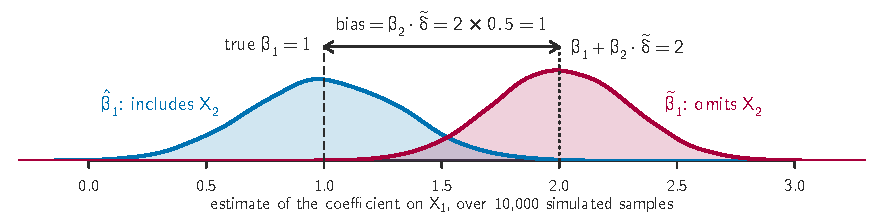
\includegraphics[width=0.85\linewidth]{ovb_sim}\par}
\slidesource{simulation with $\beta_1=1$, $\beta_2=2$, $\tilde{\delta}=0.5$, $n=50$; $X$ held fixed across 10{,}000 samples.}
}

\frame{
\frametitle{Omitted Variable Bias: Simple Case}
Direction of the bias of $\tilde{\beta}_1$ compared to $\beta_1$ is given by:
\begin{center}
\begin{tabular}{c|c|c}
   & $\cor[x_1,x_2]>0$ & $\cor[x_1,x_2]<0$ \\
   \hline
  $\beta_2>0$ & positive bias & negative bias \\
  $\beta_2<0$ & negative bias & positive bias \\
  \hline
\end{tabular}
\end{center}
\bigskip
\pause
Further points:
\begin{itemize}
  \item Magnitude of the bias matters too\pause
  \item If you miss an important confounder, your estimates are biased and inconsistent.\pause
  \item In the more general case  with $k\geq3$ the bias is more difficult to discern. It depends on all the pairwise correlations.
\end{itemize}

}

\section{Multicollinearity}

\frame{
\frametitle{Hierarchy of OLS Assumptions}

% Same diagram as in the first section, with the Gauss--Markov column
% emphasized: the next slides add Assumption V to get the variance.
\begin{center}
\olshierarchy{3}
\end{center}

}

\frame{
\frametitle{Variance of OLS Estimators}
\small
Given unbiasedness, we know the means of the sampling distributions of our OLS estimators $\hat{\beta}_j$, but we also want to know their variances.\\\medskip\pause

We could compute the variance under Assumptions I--IV, but we'll make an additional assumption to keep things tractable.\\\medskip \pause
\begin{assumption}[V. Homoskedasticity]
The error term has the same (conditional) variance given any values of the explanatory variables:
$V[u|X_1,X_2,...,X_k]=\sigma^2_u$\\\pause\medskip
This implies $V[u]=\sigma^2_u$. The constant error variance $\sigma^2_u$ measures the unseen scatter around the population regression (hyper-)plane.\\
Together the Gauss--Markov Assumptions I--V imply:\[
E[Y|X_1,...,X_k]=\beta_0 + \beta_1  X_1 +... + \beta_k X_k, \qquad
V[Y|X_1,...,X_k]=\sigma^2_u
\]
\end{assumption}\medskip
Violation: $V[u|X_1=1] \neq V[u|X_1=0]$ called \pause heteroskedasticity.
}

%\frame{
%\frametitle{Example: $V[u|X]=\sigma^2_u$ Homoscedasticity}

%\vspace{-.3cm}
%\begin{figure}[ht] \centering
%        \scalebox{.65}{\includegraphics{homo1.pdf}}
%\end{figure}

%}

%\frame{
%\frametitle{Example: $V[u|X_i]=\sigma^2_{i,u}$ Heteroscedasticity}

%\vspace{-.3cm}
%\begin{figure}[ht] \centering
%        \scalebox{.65}{\includegraphics{homo2.pdf}}
%\end{figure}

%}

\frame{
\frametitle{Variance of OLS Estimators}
The variance expression is also similar to the simple regression case. \pause
\begin{theorem}[Variance of OLS Estimators]
Given OLS Assumptions I--V (Gauss-Markov Assumptions):
$$
\var[\hat{\beta}_j\mid X]=\frac{\sigma_u^2}{\sum_{i=1}^n (x_{i,j} - \bar{x}_j)^2(1-R_j^2)}=\frac{\sigma_u^2}{SST_j(1-R_j^2)}
$$
for $j=1,2$, where $R_j^2$ is the R-squared from regression of $X_j$ on the other $X$ variable and a constant.
\end{theorem}
\begin{proof}
Analogous to the proof for the simple regression case, but algebraically cumbersome. See Wooldridge Chapter 3 Appendix for details. \\
(We'll cover a more general case of $K$ regressors using matrices, which makes the derivation much simpler.)
\end{proof}
}


\frame{
\frametitle{Estimating $\sigma^2$ to get Standard Errors}
\small
To estimate the OLS variance, we first need to estimate \pause $\sigma^2_u$, as in the simple regression case. \pause
\begin{theorem}[Unbiased Estimation of the Error Variance]
Given OLS Assumptions I--V, to estimate the error variance $\sigma^2_u$ we use our unbiased estimator $\hat{\sigma}_u^2$:
$$
\hat{\sigma}_u^2 = \frac{1}{n-3}\sum_{i=1}^n \hat{u}_i^2=\frac{SSR}{n-3}
$$
\end{theorem}
\begin{proof}
Analogous to the simple regression case. We'll revisit the proof using matrices.
\end{proof}
\begin{itemize}
    \item $\hat\sigma_u$ is often called the \alert{residual standard error} of the regression.
    \item $n-3$ is the \alert{degrees of freedom}.
    \item When $k>2$, the degrees of freedom $= n - k - 1$, or
      $(\text{\# of observations}) - (\text{\# of estimated parameters})$.
\end{itemize}
}

\frame{
\frametitle{Estimating the Variance of OLS Estimators}

Given our unbiased estimator for the error variance $\sigma^2$:
$$
\hat{\sigma}_u^2 = \frac{\sum_{i=1}^n \hat{u}_i^2}{n-3}=SSR/(n-3)
$$
we can estimate the \alert{standard errors} of our regression coefficients as
$$
\widehat{SE}[\hat{\beta}_j] = \sqrt{\widehat{V}[\hat{\beta}_j]} = \frac{\hat{\sigma}_u}{\sqrt{ \sum_{i=1}^n(x_{i,j} - \bar{x}_j)^2(1-R_j^2) }}
$$

\pause
The Gauss-Markov Theorem: Given OLS Assumptions I--V, the multiple OLS estimator is \alert{BLUE}.
}

% Output reproduced by code/residual_se.R (code/residual_se_output.txt):
% the Lecture 5-1 running example, model (2).
\begin{frame}[fragile]
\frametitle{Example: Executive Corruption on Court Independence and Democracy}

\spacingset{0.8}
\begin{Verbatim}[fontsize=\footnotesize, frame=single, label=R Code, commandchars=\\\{\}]
> fit <- lm(execorr100 ~ courtind + democracy, data = d)
> summary(fit)

~~~~~

Coefficients:
            Estimate \textcolor{red}{Std. Error} t value Pr(>|t|)
(Intercept)   78.324      \textcolor{red}{3.593}  21.799  < 2e-16 ***
courtind     -10.630      \textcolor{red}{2.113}  -5.031 1.27e-06 ***
democracy    -21.510      \textcolor{red}{4.672}  -4.604 8.22e-06 ***
---
Signif. codes:  0 *** 0.001 ** 0.01 * 0.05 . 0.1   1

\textcolor{red}{Residual standard error: 20.92 on 165 degrees of freedom}
Multiple R-squared: 0.5039,	Adjusted R-squared: 0.4978
F-statistic: 83.78 on 2 and 165 DF,  p-value: < 2.2e-16
\end{Verbatim}
\pause
\medskip
\begin{Verbatim}[fontsize=\footnotesize, frame=single, label=R Code, commandchars=\\\{\}]
> DF <- nrow(d) - length(coef(fit))  # = DF of the regression
> DF
[1] 165
>
> sqrt(sum(residuals(fit)^2) / DF)  # = residual standard error
[1] 20.91745
\end{Verbatim}
\slidesource{V-Dem v16, 2024, 168 countries, as in Lecture 5-1. execorr100: V-Dem's executive corruption index times 100 (0 = clean); courtind: high court independence (0 = never, 4 = always); democracy: electoral democracy index above 0.5.}

\end{frame}

\frame{
\frametitle{Three Components of the OLS Variance Estimators}

$$
V[\hat{\beta}_j\mid X]=\frac{\sigma^2_u}{\sum_{i=1}^n (x_{i,j} - \bar{x}_j)^2(1-R_j^2)}=\frac{\sigma_u^2}{SST_j(1-R_j^2)}
$$
%Note that this shows why including an irrelevant variable inflates $V[\hat\beta_j\mid X]$.\\
%\pause
\smallskip
When will the variance be large? \\
\pause
Notice the three components of the variance:
\begin{enumerate}
  \item $\sigma^2_u$ is the \alert{error variance}, the unseen scatter around the population regression plane. The OLS variance is increasing in $\sigma_u^2$. \medskip\pause
  \item $SST_j$ is the \alert{total sample variation in $x_j$}, which equals:
    $$ SST_j \ = \ n\cdot \frac{1}{n}\sum_{i=1}^n (x_{i,j}-\bar{x}_j)^2 \ = \ n \cdot MSD(x_j).$$
    So the OLS variance is decreasing in sample size and spread of $x_j$.\smallskip\pause
  \item $R_j^2$ measures the \alert{strength of linear relationship between the
  explanatory variables}. The OLS variance is increasing in $R_j^2$.
\end{enumerate}
}


\frame{
\frametitle{Multicollinearity and Collinearity}

\begin{itemize}
\item Multicollinearity occurs if two or more explanatory variables are strongly correlated.
That is, when $R_j^2$ is large. \medskip \pause
\item We know that (perfect) \alert{collinearity} violates our regression assumptions and OLS breaks down. What does collinearity imply about $R_j^2$? \pause \quad $R_j^2=1$, which implies
$$ V[\hat{\beta}_j\mid X] \ = \ \frac{\sigma^2_u}{SST_j(1-R_j^2)}
 \ = \ \frac{\sigma^2_u}{SST_j(1-1)} \ = \ \frac{\sigma^2_u}{0} $$
    \pause
\item Therefore, OLS breaks down when $R_j^2=1$ (perfect collinearity).
\item If $R_j^2 \approx 1$ (multicollinearity), OLS does NOT break down; it just has
a very high standard error.
\end{itemize}

}

\frame{
\frametitle{How Do We Detect Multicollinearity?}
\small
\begin{itemize}
\item The best practice is to directly compute $\cor(X_1,X_2)$ before running your regression.
\pause
\medskip
\item Warning signs in the regression output (none proves multicollinearity; the first is also what omitted variable bias looks like):
\begin{itemize}
\item Large changes in the estimated regression coefficients when a predictor variable is added or deleted\medskip
\item Lack of statistical significance despite high $R^2$\medskip
\item Estimated regression coefficients have an opposite sign from predicted
\end{itemize}
\pause
\item A more formal indicator is the \alert{variance inflation factor (VIF)}:
$$VIF(\beta_j)=\frac{1}{1-R_j^2}$$
which measures how much $V[\hat\beta_j\mid X]$ is inflated compared to (hypothetical)
uncorrelated data. \\
\pause
In R, \texttt{vif()} in the {\tt car} package.
\end{itemize}

}


\frame{
\frametitle{Multicollinearity: Simulation Example}

\begin{itemize}
\item So how serious is the multicollinearity problem in practice? Let's find out by simulation.
\pause
\medskip
\item The model: $Y=\beta_0+\beta_1 X_1 + \beta_{2} X_2 + u$\pause
\item Vary $R_1^2$, the squared correlation between $X_1$ and $X_2$. Fix $n$ at 50.
\item See what happens to the standard error of $\hat{\beta}_1$
\end{itemize}
\pause
% Numbers from code/fig_multicollinearity.R (saved in code/fig_multicollinearity_table.txt).
\begin{table}
\begin{center}
\begin{tabular}{|l|l|l|l|l|l|}
\hline
  {\bf $R_1^2$ } &          0 &          .5 &          .75 &          .9 &          .99 \\
\hline
{\bf SE($\hat{\beta}_1$) } &          0.144 &          0.204 &          0.288 &          0.454 &          1.429 \\
\hline
{\bf SE ratio to $R_1^2=0$ } &          1.00 &          1.42 &          2.01 &          3.16 &         9.95 \\
\hline
{\bf $\sqrt{VIF}=1/\sqrt{1-R_1^2}$ } &          1.00 &          1.41 &          2.00 &          3.16 &         10.00 \\
\hline
\end{tabular}
\end{center}
\end{table}

So the standard error doubles at $R_1^2=.75$, more than triples (about 3.2 times) at $.9$, and grows tenfold at $.99$: modest correlations cost little, but the cost explodes as $R_1^2\to1$.
\slidesource{simulation with $\beta_1=\beta_2=1$, $u\sim N(0,1)$. Each column: 10{,}000 samples, with $X$ fixed and only $u$ redrawn. Columns differ only in $x_2$, which sets $R_1^2$.}

}

\frame{
\frametitle{Variance Inflation due to Multicollinearity ($k=2$)}

\vspace{-.3cm}
\begin{figure}[ht] \centering
        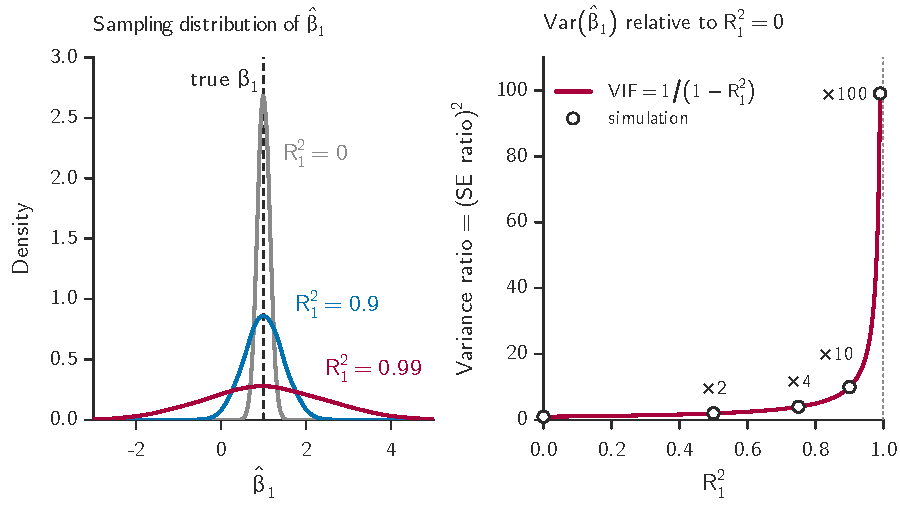
\includegraphics[height=0.82\textheight]{multicollinearity_variance}
\end{figure}

}

% Numbers and figure from code/fig_multicollinearity_vdem.R (code/multicollinearity_vdem_output.txt).
\frame{
\frametitle{Multicollinearity: Two Measures of Democracy}
\small
Executive corruption (0--100) on V-Dem's electoral democracy index (polyarchy) and liberal democracy index (libdem), 179 countries in 2024.
\begin{columns}[T]
\begin{column}{0.36\textwidth}
\centering
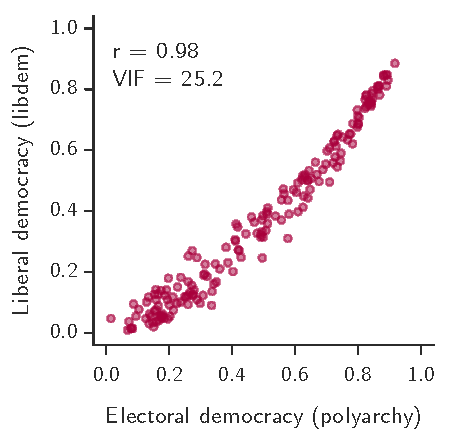
\includegraphics[width=\linewidth]{polyarchy_libdem}
\end{column}
\begin{column}{0.62\textwidth}
\begin{center}
\begin{tabular}{lccc}
\hline
 & alone & alone & together \\
\hline
polyarchy & $-82.6$ (5.9) & & $+130.5$ (24.5) \\
libdem & & $-89.2$ (5.2) & $-216.6$ (24.4) \\
\hline
\end{tabular}\\[2pt]
{\footnotesize Standard errors in parentheses.}
\end{center}
\pause
\begin{itemize}
\item $\cor(\text{polyarchy},\text{libdem})=.980$, so $R_j^2=.96$ and $VIF=25.2$.
\item Together, the standard errors grow about 4 to 5 times ($\sqrt{VIF}=5.0$, partly offset by a smaller $\hat{\sigma}_u$). The signs split. Polyarchy turns positive.
\item Both slopes are still significant ($t=5.3$ and $-8.9$). The warning sign here is the sign flip.
\end{itemize}
\pause
Why? V-Dem builds libdem from polyarchy plus a liberal component. The data have almost no countries that differ in one index at the same value of the other, so OLS cannot pull the two apart.
\end{column}
\end{columns}
\slidesource{V-Dem v16, 2024. The codebook says the liberal democracy index ``also takes the level of electoral democracy into account.''}
}

\frame{
\frametitle{So How Should I Think about Multicollinearity?}

\begin{itemize}
\item Multicollinearity does NOT lead to bias; estimates will be unbiased and consistent.\pause
\item Multicollinearity should in fact be seen as a problem of \alert{micronumerosity} (Goldberger 1991), that is, too little data. You can't ask the OLS estimator to distinguish
the partial effects of $X_1$ and $X_2$ if they are essentially the same.\pause
\item If $X_1$ and $X_2$ are almost the same, why would you want a unique $\beta_{1}$ and a unique $\beta_{2}$? Think about how you would interpret that?
\medskip
\pause
\item Relax, you got way more important things to worry about!
\item If possible, get more data
\item Drop one of the variables (if its true coefficient is not zero, this brings back omitted variable bias), or combine them into one index
\item Or maybe linear regression is not the right tool

\end{itemize}

}

% \frame{
% \frametitle{What Should I do to tackle multicollinearity?}

% \begin{itemize}
% \item Get more data!\\\medskip\pause
% \item Drop one variable.\\\medskip\pause
% \item Or combine them.\\\medskip\pause
% \item Go non-parametric: Matching, etc.! \\
% (You need to wait until Quant II to appreciate this one.)\medskip\pause
% \item And always remember: the $V[\beta_j]$ depends on the \alert{interplay} of $\sigma^2_u$, $R_j^2$, and $SST_j$.
% \end{itemize}

% }

%\frame{
%\frametitle{Variance in Misspecified Models}
%$$
%V[\hat{\beta}_j]=\frac{\sigma^2}{\sum_{i=1}^n (x_i - \bar{x})^2(1-R_j^2)}=\frac{\sigma^2}{SST_j(1-R_j^2)}
%$$
%
%}

%\section{Testing and Confidence Intervals}


%\frame{
%\frametitle{Testing and Confidence Intervals}

%Three potentials goals for regression:
%\begin{enumerate}
%\item Point Estimation: Consider the sampling distribution of a point estimator\medskip
%\item Hypothesis Testing: Consider the sampling distribution of a test statistic to test hypothesis about $\beta_j$ at the $\alpha$ level \medskip
%\item Interval Estimation: Consider the sampling distribution of an interval estimator to construct intervals that will contain $\beta_j$ at least $1-\alpha$ of the time.
%\end{enumerate}\medskip
%Notice: For 2-3 we need to know more than just the mean and the variance of the sampling distribution of $\hat{\beta}_j$. We need to know the shape of the full sampling distribution.

%}

%\subsection{Small Sample}

%\frame{

%\frametitle{OLS Assumptions VI}
%\small
%\begin{assumption}[VI. Normality]

%The error term is independent of all explanatory variables and is normally distributed with mean zero and variance $\sigma^2_u$: $u_i \sim N(0,\sigma^2)$ which implies$$
%Y|X_1,X_2,...,X_k \sim N(\beta_0+\beta_1 X_1,...,+\beta_k X_k,\sigma^2_u)
%$$
%Notice: This implies homoscedasticity and zero conditional mean.
%\end{assumption}\medskip \pause
%\begin{itemize}
%  \item Together assumptions 1-6 are called the \alert{classical linear model assumptions}\pause
%  \item Non-normality of the errors is a serious concern in small samples (transformation of the variables can help)\pause
%  \item Non-normality of the errors is not a serious concerns in large samples because we can rely on the central limit theorem.
%\end{itemize}

%}

%\frame{
%\frametitle{Sampling Distribution for $\widehat{\beta}_j$}
%\small
%\begin{theorem}[Sampling Distribution of $\widehat{\beta}_j$]
%Under assumptions 1-6,
%$$
%\widehat{\beta}_j \sim N\left(\beta_j, V[\widehat{\beta}_j]\right)
%$$\pause
%$$
%SE[\hat{\beta}_j] =  \frac{\sigma}{\sqrt{ \sum_{i=1}^n(x_{i,j} - \bar{x}_j)^2(1-R_j^2) }}
%$$\pause
%$$
%\frac{\widehat{\beta}_j - \beta_j}{SE[\hat{\beta}_j]} \sim N(0,1)
%$$
%\end{theorem}\pause
%%Notice:
%%\begin{itemize}
%%\item $\beta_1$ is the unknown parameter of interest.
%%\item $\sigma$ is also unkown. Parameter helps us describe the sampling distribution of $\widehat{\beta}_1$ (nuisance parameter)
%%\end{itemize}
%\vspace{-.1cm}
%\begin{proof}
%Analogous to k=1 case. Given 1-6, $\widehat{\beta}_j$ is just a linear combination of the errors which are independent normals. Any linear combination of independent normals is normal and we can transform any normal into a standard normal.
%\end{proof}

%}

%\frame{
%\frametitle{The t-Test for Single Population Parameters}

%\begin{footnotesize}
%\begin{theorem}[Sampling Distribution of t-value]
%$SE[\hat{\beta}_j] =  \frac{\sigma}{\sqrt{ \sum_{i=1}^n(x_{i,j} - \bar{x}_j)^2(1-R_j^2) }}$ involves the standard error of the regression $\sigma$. Since we also need to estimate this using $\hat{\sigma}^2 = \frac{\sum_{i=1}^n \hat{u}_i^2}{n-k-1}$ we have that under assumptions 1-6, the so called \alert{t-value} is characterized by:
%$$
%\frac{\widehat{\beta}_j - \beta_j}{\widehat{SE[\hat{\beta}_j]}} \sim t_{n-k-1}
%$$
%\end{theorem}\pause
%\begin{proof}
%Analogous to k=1 case.
%\end{proof}
%\end{footnotesize}
%}


%\frame{
%\frametitle{Using the t-Value as a Test Statistic}
%\begin{footnotesize}
%$$
%\frac{\widehat{\beta}_j - c}{\widehat{SE[\hat{\beta}_j]}} \sim t_{n-k-1}
%$$
%\begin{enumerate}
%\item Assuming some \alert{null value} $c$ (e.g. $c=0$ refers to $H_0$: $\beta_j=0$) and given the number of observations we know that the sampling distribution of this test statistic is $t_{n-k-1}$. \alert{This is the only difference to the $k=1$ case where $t_{n-2}$} \medskip \pause
%\item So we know the probability that the value of our test statistics falls into a given interval:
%$$
%P\left(  -t_{\alpha/2}   \le     \frac{\widehat{\beta}_j - \beta_j}{\widehat{SE[\hat{\beta}_j]}}  \le  t_{\alpha/2} \right)= 1- \alpha
%$$\medskip \pause
%\item Since we can also estimate $\widehat{\beta}_j$ and $\widehat{SE[\hat{\beta}_j]}$ we can easily compute the realized t-value in our application.\medskip \pause
%\item We can then check if the realized value is ``unusual'' given the known distribution of the test statistic. We reject $H_0$ or not or report a p-value.
%    \end{enumerate}
%\end{footnotesize}

%}

%\frame{
%\frametitle{Confidence Intervals}
%\begin{footnotesize}
%To construct confidence intervals, there is again no difference compared to the case of $k=1$, except that we need to use $t_{n-k-1}$ instead of $t_{n-2}$\\\medskip Since we know the sampling distribution for our t-value:
%$$
%\frac{\widehat{\beta}_j - \beta_j}{\widehat{SE[\hat{\beta}_j]}} \sim t_{n-k-1}
%$$\pause
%So we also know the probability that the value of our test statistics falls into a given interval:
%\begin{align*}
%P\left(  -t_{\alpha/2}   \le     \frac{\widehat{\beta}_j - \beta_j}{\widehat{SE[\hat{\beta}_j]}}  \le  t_{\alpha/2} \right) &= 1- \alpha \\
%%P(  -t_{\alpha/2}\widehat{SE[\hat{\beta}_1]}   <     \widehat{\beta}_1 - \beta_1 <  t_{\alpha/2}\widehat{SE[\hat{\beta}_1]} ) &= 1- \alpha \\
%%P(  -t_{\alpha/2}\widehat{SE[\hat{\beta}_1]} - \widehat{\beta}_1 <   - \beta_1 <  t_{\alpha/2}\widehat{SE[\hat{\beta}_1]}  -\widehat{\beta}_1) &= 1- \alpha \\
%%P\left(   \widehat{\beta}_1-t_{\alpha/2}\widehat{SE[\hat{\beta}_1]}  \le    \beta_1 \le  \widehat{\beta}_1 + t_{\alpha/2}\widehat{SE[\hat{\beta}_1]}  \right) &= 1- \alpha
%\end{align*}\pause
%We rearrange:$$
%[ \widehat{\beta}_1-t_{\alpha/2}\widehat{SE[\hat{\beta}_1]}\,,\,\widehat{\beta}_1 + t_{\alpha/2}\widehat{SE[\hat{\beta}_1]}]
%$$\\\medskip\pause
%and thus can construct the confidence intervals as usual using:
%$$
%\hat{\beta}_j \pm t_{\alpha/2} \cdot \widehat{SE}[\hat{\beta}_j]
%$$
%\end{footnotesize}
%}

%\frame{
%\frametitle{Example: Democracy on GDP, Heterogeneity, and Colony}

%\vspace{-.3cm}
%\begin{figure}[ht] \centering
%        \scalebox{.65}{\includegraphics{model.pdf}}
%\end{figure}

%}

%\frame{
%\frametitle{Hierarchy of OLS Assumptions}

%\vspace{-.3cm}
%\begin{figure}[ht] \centering
%        \scalebox{.45}{\includegraphics{assumptionsfig.pdf}}
%\end{figure}

%}

%\subsection{Large Sample}

%\frame{
%\frametitle{Large Sample Properties: Consistency}

%\begin{footnotesize}
%\begin{theorem}[Consistency of OLS Estimator]
%Given assumptions 1-4 the OLS estimator $\widehat{\beta}_j$ is consistent for $\beta_j$. We can write this as:$$
%\mbox{plim } \widehat{\beta}_{j,n} = \beta_j
%$$
%for all $j=0,...,k$. Notice: We can relax $E[u|X_1,...,X_k]=0$ to $COV[u,X_j]=0$ for all $j$.
%\end{theorem}\pause
%\begin{proof}
%Similar to the $k=1$ case. Recall:\\
%$\mbox{plim } \widehat{\beta}_{1,n}=  \beta_{1,n} + \mbox{plim } \frac{n^{-1}\sum_i^n (x_i - \bar{x})u_i }{n^{-1}\sum_i^n (x_i - \bar{x})^2}$ (true value and limiting value of the error term)\\\pause
%$\mbox{plim } \widehat{\beta}_{1,n} = \beta_1 + \frac{COV[X,u]}{V[X]}$ (by a LLN the sample quantities converge in probability)\\\pause
%$\mbox{plim } \widehat{\beta}_{1,n} = \beta_1$ (given $COV[X,u]=0$ and $V[X]>0$)\\\medskip
%Full proof for multivariate case requires matrix algebra.
%\end{proof}
%\end{footnotesize}

%}


%\frame{
%\frametitle{Large Sample Inference}

%\begin{footnotesize}
%\begin{theorem}[Asymptotic Normality of OLS Estimator]
%For testing we need to know the full sampling distribution of the estimator. Fortunately, given assumptions 1-5 the OLS estimator $\widehat{\beta}_j$ is asymptotically normally distributed:
%$$
%\frac{\hat{\beta}_{j,n} - \beta_j}{SE[\hat{\beta}_{j,n}]} \stackrel{d}{\rightarrow} N(0,1)$$
%$$
%\widehat{V[\hat{\beta}_{j,n}]}= \frac{\sigma^2_u}{ \sum_{i=1}^n(x_{i,j} - \bar{x}_j)^2(1-R_j^2) } \mbox{ with consistent estimator }  \hat{\sigma}^2_{u,n}=\frac{1}{n-k-1}\sum_{i=1}^n \hat{u}_i^2 \stackrel{p}{\rightarrow} \sigma^2_u
%$$
%\end{theorem}\pause
%\begin{proof}
%Analogous to k=1 case, but full proof is somewhat involved. Intuition is that errors are sequence of iid. RVs with mean zero and variance $\sigma^2_u$ so their scaled mean converges in distribution to a normal $N(0,\sigma^2_u)$ by the CLT and our estimator is a linear combination of normals.
%\end{proof}\pause
%\begin{itemize}
%  \item We need homoscedasticity for this result, but we can drop normality. So \alert{asymptotic} standard errors, t-values, p-values, and CIs remain valid!
%%  \item As $n\rightarrow\infty$ $V[\hat{\beta}_j] \rightarrow 0$ at a rate of $1/n$
%%  \item Under 1-5 this asymptotic variance is also the lowest in class (Gauss-Markov).
%\end{itemize}
%\end{footnotesize}

%}



\section{Including an Irrelevant Variable}


\frame{
\frametitle{Including an Irrelevant Variable: Simple Case}

\alert{True Population Model}:
$$
y = \beta_0 + \beta_1 x_1 + \beta_2 x_2 + u \quad \text{where} \quad \beta_2 = 0
$$ and Assumptions I--IV hold.\\\medskip
\alert{Overspecified Model} that we use:
$$
\hat{y} = \hat{\beta}_0 + \hat{\beta}_1 x_1 + \hat{\beta}_2 x_2
$$
Q: Which statement is correct?
\begin{enumerate}
  \item $E[\hat{\beta}_1] > \beta_1$
  \item $E[\hat{\beta}_1] < \beta_1$
  \item $E[\hat{\beta}_1] = \beta_1$
  \item Can't tell
\end{enumerate}
}

\frame{
\frametitle{Including an Irrelevant Variable: Simple Case}

Recall: Given Assumptions I--IV, we have:
$$
E[\hat{\beta}_j]=\beta_j
$$
for \alert{all} values of $\beta_j$. So, if $\beta_2=0$, we get
$$
E[\hat{\beta}_0]=\beta_0,\, E[\hat{\beta}_1]=\beta_1,\,E[\hat{\beta}_2]=0
$$
and thus including the irrelevant variable does not affect the unbiasedness. The sampling distribution of $\hat{\beta}_2$ will be centered about zero.\\\medskip\pause

But under Assumption V (homoskedasticity), including an irrelevant variable increases the variance of $\hat\beta_1$ (unless $x_2$ is uncorrelated with $x_1$ in the sample, so that $R_1^2=0$), because\\
  \[
  V[\hat\beta_1\mid X]=\frac{\sigma_u^2}{SST_1(1-R_1^2)}\ \ge\ \frac{\sigma_u^2}{SST_1}=V[\tilde\beta_1\mid X],\qquad R_1^2\equiv R^2\text{ from regressing }x_1\text{ on }(1,x_2),
  \]
where $\tilde\beta_1$ is the slope from the correct simple regression of $y$ on $x_1$.

%You can cook up examples where it actually does lead to bias (M-bias), but this is empirically rare.

}

% \frame{
% \frametitle{Including an Irrelevant Variable: Simple Case}

% \textbf{Worksheet Q2}\medskip

% Suppose the true model is $y=\beta_0+\beta_1 x_1+u$ and Assumptions I–V hold. You nevertheless estimate the overspecified model $\tilde y=\tilde\beta_0+\tilde\beta_1 x_1+\tilde\beta_2 x_2$, where $x_2$ is correlated with $x_1$ but is irrelevant in truth ($\beta_2=0$).

% \begin{enumerate}
%   \item Show that $E[\hat{\beta}_0]=\beta_0,\, E[\hat{\beta}_1]=\beta_1,\,E[\hat{\beta}_2]=0$.  
%   \item Explain that the conditional variance inflates according to
%   \[
%   V[\tilde\beta_1\mid X]=\frac{\sigma_u^2}{SST_1(1-R_1^2)},\qquad R_1^2\equiv R^2\text{ from regressing }x_1\text{ on }(1,x_2),
%   \]
%   and compare to the variance in the correctly specified simple regression, $V[\hat\beta_1^{(SR)}\mid X]=\sigma_u^2/SST_1$.  
% \end{enumerate}

% }

\end{document}
